\testfile{pgfplotstest.misc.tex}

\testsection{Paths after addplot}
\testsubsection{plot coordinates}
\testsubsubsection{without space after 'coordinates'}
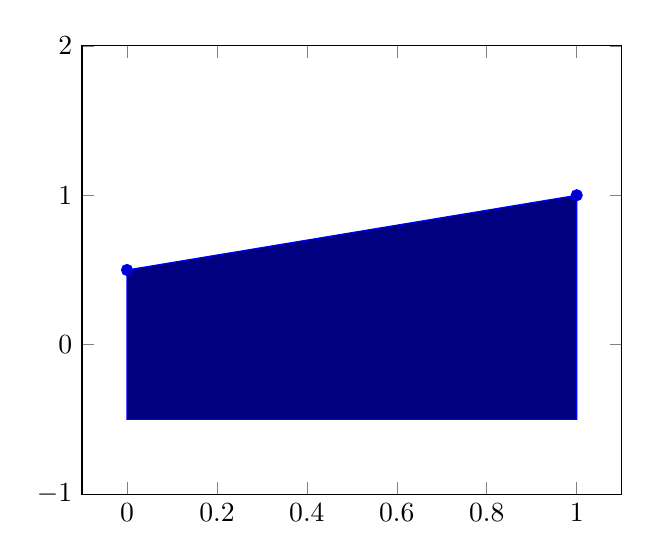
\begin{tikzpicture}
\begin{axis}[ymin=-1,ymax=2]
\addplot+[fill=blue!50!black] coordinates{(0,0.5) (1,1)} |- (axis cs:0,-0.5) -- cycle;
\end{axis}
\end{tikzpicture}

\testsubsubsection{with space after 'coordinates'}
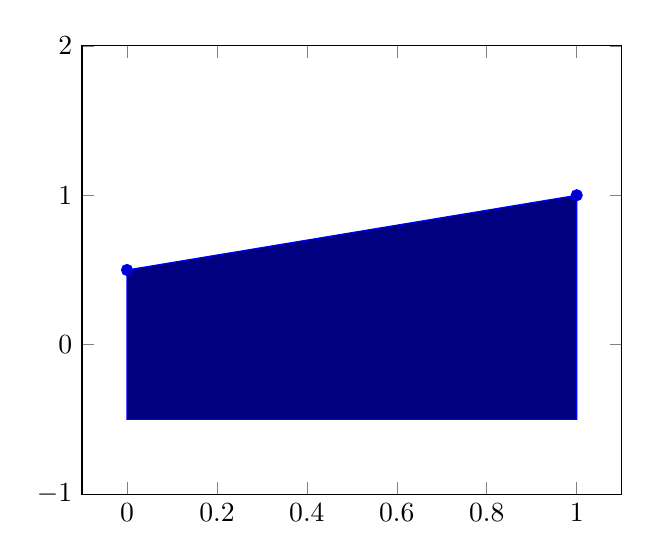
\begin{tikzpicture}
\begin{axis}[ymin=-1,ymax=2]
\addplot+[fill=blue!50!black] coordinates {(0,0.5) (1,1)} |- (axis cs:0,-0.5) -- cycle;
\end{axis}
\end{tikzpicture}

\testsubsubsection{using closedcycle path}
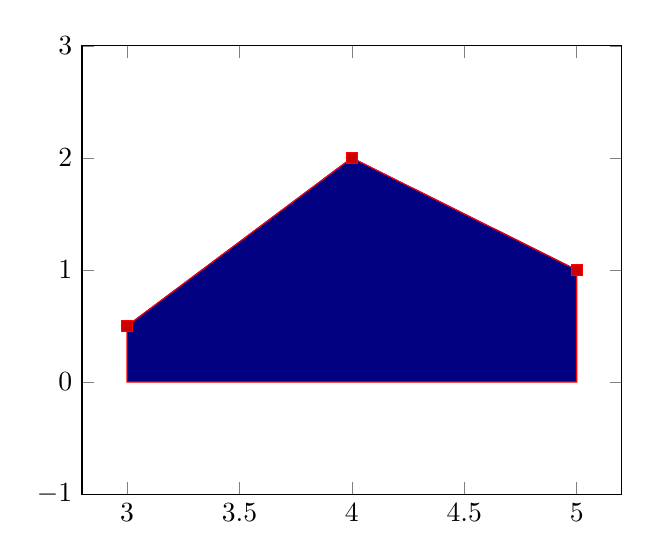
\begin{tikzpicture}
\begin{axis}[ymin=-1,ymax=3]
\addplot coordinates {(3,0.5) (4,2) (5,1)} ;
\addplot+[fill=blue!50!black] coordinates {(3,0.5) (4,2) (5,1)} 
	\closedcycle;
\end{axis}
\end{tikzpicture}

\testsubsection{plot table}
\begin{tikzpicture}
\begin{axis}
\addplot+[fill=blue!50!black] table[x index=0,y index=1,header=false]{plotdata/pgfplotstest_plot2.gnuplot} |- (axis cs:0,-1) -- cycle;
\end{axis}
\end{tikzpicture}

\testsubsection{plot function}
\begin{tikzpicture}
\begin{axis}
\addplot plot[id=parable,domain=-5:5] function{4*x**2 - 5} node[pin=180:{$4x^2-5$}]{};
\end{axis}
\end{tikzpicture}


\testsection{Title-option}
\begin{tikzpicture}
\begin{loglogaxis}[title=A test title,xlabel=Dof,ylabel=Error]
\loglogtestplot
\end{loglogaxis}
\end{tikzpicture}

\testsection{Filter test}
{%
\def\myOwnYfilter#1\to#2{%
	\def#2{0.5}%
}%
\begin{tikzpicture}
%
\begin{axis}[yfilter={\myOwnYfilter}]
\addplot plot coordinates {
	(4,0)
	(6,1)
};
\end{axis}
\end{tikzpicture}

\begin{tikzpicture}
\begin{axis}[y filter/.code={\def\pgfmathresult{0.5}}]
\addplot plot coordinates {
	(4,0)
	(6,1)
};
\end{axis}
\end{tikzpicture}

\begin{tikzpicture}
\begin{axis}[x filter/.code={\ifnum\coordindex>4\def\pgfmathresult{}\fi}]
\addplot (\x,\x^2);
\end{axis}
\end{tikzpicture}
}%

\testsection{Test for addplot+[...]}
{
\pgfplotsset{every axis legend/.append style={at={(1.03,1)},anchor=north west}}
\begin{enumerate}
	\item Ohne aenderung:

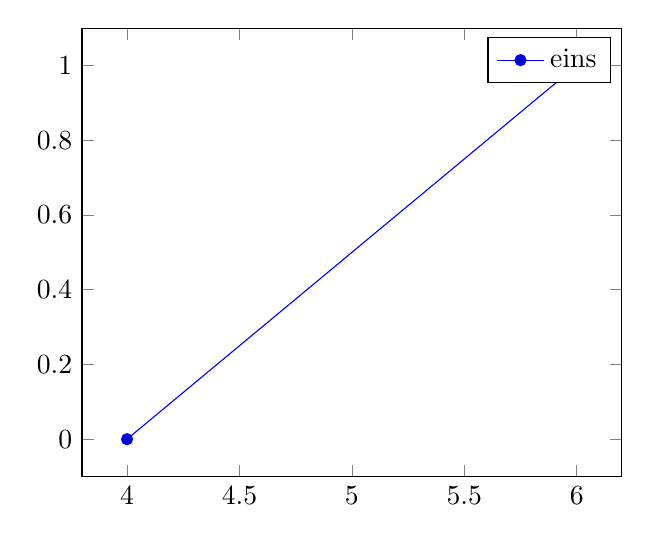
\begin{tikzpicture}
\begin{axis}
\smallplotstest

\addplot plot coordinates {
	(4,0)
	(6,1)
};
\legend{eins\\zwei\\}%
\end{axis}
\end{tikzpicture}

\item MIT aenderung:

\begin{tikzpicture}
\begin{axis}
\smallplotstest

\addplot+[only marks] plot coordinates {
	(4,0)
	(6,1)
};
\legend{eins\\zwei\\}%
\end{axis}
\end{tikzpicture}
\end{enumerate}
}

\testsection{Hide axis test}
\begin{tikzpicture}
	\begin{axis}
		\smallplotstest
	\end{axis}
\end{tikzpicture}
\begin{tikzpicture}
	\begin{axis}[hide axis]
		\smallplotstest
	\end{axis}
\end{tikzpicture}
\vskip 1cm
\noindent
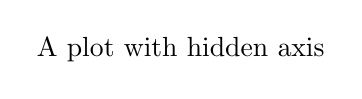
\begin{tikzpicture}
	\begin{axis}[hide axis,title=A plot with hidden axis]
		\smallplotstest
	\end{axis}
\end{tikzpicture}
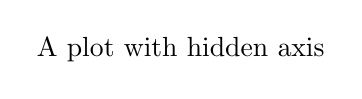
\begin{tikzpicture}
	\begin{axis}[hide axis,title=A plot with hidden axis]
		\smallplotstest
		\legend{A legend\\}
	\end{axis}
\end{tikzpicture}

{
\def\testaxis#1{
	\begin{tikzpicture}
	\begin{axis}[#1,title=A title,xlabel=$x$,ylabel=$y$]
	
	\addplot (\x,\x^2);
	\legend{$x^2$}
	\end{axis}
	\end{tikzpicture}
}
\testsubsection{hide x/y axis}
\testaxis{hide x axis}

\testaxis{hide y axis}

\testaxis{hide x axis,axis y line=center}

\testaxis{hide y axis,axis x line=center}

\testaxis{hide x axis,axis y line=right}

\testaxis{hide y axis,axis x line=bottom}
}

\testsection{disabledatascaling / disablelogfilter}
\testsubsection{disabledatascaling}
\begin{tikzpicture}
\begin{axis}[disabledatascaling]
	\smallplotstest
\end{axis}
\end{tikzpicture}

\testsubsection{disabledatascaling+circle at $(0,0)$ radius $(0.5)$}
\begin{tikzpicture}
\begin{axis}[disabledatascaling]
	\smallplotstest

	\draw (0,0) circle (0.5);
\end{axis}
\end{tikzpicture}

\testsubsection{disabledatascaling + explicit limits}
\begin{tikzpicture}
\begin{axis}[disabledatascaling, xmin=0, xmax=1, ymin=0, ymax=1]
	\smallplotstest
\end{axis}
\end{tikzpicture}

\testsubsection{disabledatascaling + explicit limits + error bars}
\begin{tikzpicture}
\begin{axis}[disabledatascaling, xmin=-0.5, xmax=1.5, ymin=-0.5, ymax=1.5]
\addplot plot[
	/pgfplots/error bars/.cd,
	y dir=both,y explicit,
	x dir=both,x fixed relative=0.5,
	error mark=diamond*,
]
	coordinates
	{(0,0) +- (0.5,0.1) 
	(0.1,0.1)  +- (0.05,0.2)
	(0.2,0.2) 	+- (0,0.05)
	(0.5,0.5)
	(1,1)};
\end{axis}
\end{tikzpicture}

\testsubsection{Reading nan und inf in linear axis}
\begin{tikzpicture}
	\begin{axis}
	\addplot coordinates {(0,0) (inf,3) (3,nan) (1,1)};
	\end{axis}
\end{tikzpicture}


\begin{tikzpicture}
	\begin{axis}[
		xmin=1600000000,
		xmax=1680000000]

	\addplot plot coordinates {
		(1602240784,0.9982)
		(1680016144,1.12698)
	};
	\end{axis}
\end{tikzpicture}

\testsubsection{check for special limit cases}
\begin{tikzpicture}
	\begin{axis}[
		clip limits=false,
		xmin=10]

	\addplot plot coordinates {
		(0,0) (1,1) (2,3)
	};
	\end{axis}
\end{tikzpicture}

\testsection{interrupt bounding box}
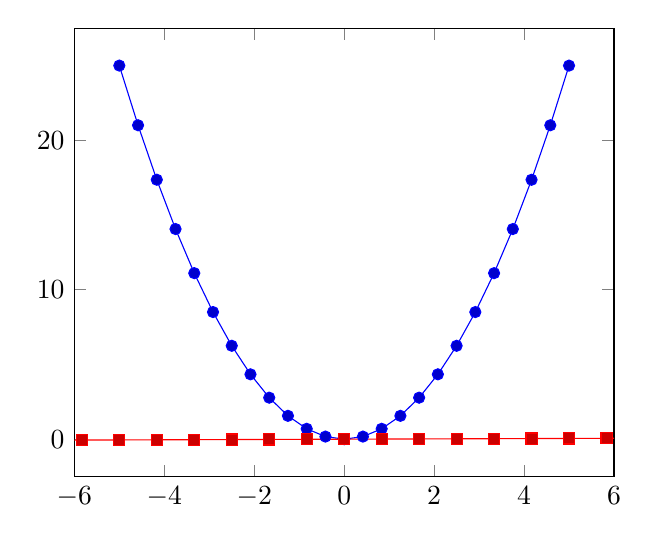
\begin{tikzpicture}
	\begin{axis}
	\addplot (\x,\x^2);

	\begin{pgfplotsinterruptdatabb}
	\addplot plot[domain=-10:10] (\x,0.01*\x);
	\end{pgfplotsinterruptdatabb}
	\end{axis}
\end{tikzpicture}

\begin{tikzpicture}
	\begin{loglogaxis}
	\addplot (\x,\x^2);

	\begin{pgfplotsinterruptdatabb}
	\addplot plot[domain=-10:10] (\x,0.01*\x);
	\end{pgfplotsinterruptdatabb}
	\end{loglogaxis}
\end{tikzpicture}

\testsection{strcmp}
{
	\def\testit#1#2{%
		\begingroup
		\pgfplotsutilstrcmp{#1}{#2}%
		\ttfamily #1 \ifcase\pgfplotsretval =\or<\or>\fi\space #2 
		\endgroup
		\par
	}%

	\testit{z}{aaa}
	\testit{A longer Test}{A longer verification}
	\testit{a}{a}
	\testit{a}{b}
	\testit{b}{a}
	\testit{aa}{ab}
	\testit{aba}{abb}
	\testit{eins}{zwei}
	\testit{vier}{fuenf}

	\pgfplotstableread{
		The
		values
		of
		these
		keys
		contain
		the
		size
		of
		the
		parent
		axis.
		They
		can
		be
		used
		as
		|width|
		and/or
		|height|
		arguments
		for
		|every
		colorbar|
		with
		|\pgfkeysvalueof{/pgfplots/parent
		axis
		width}|.
		These
		values
		are
		only
		valid
		inside
		of
		color
		bars.
		\end{pgfplotskeylist}
		Besides
		these
		values,
		each
		color
		bar
		inherits
		a
		list
		of
		styles
		of
		its
		parent
		axis,
		namely
		\begin{itemize}
		\item
		|every
		tick|,
		\item
		|every
		minor
		tick|,
		\item
		|every
		major
		tick|,
		\item
		|every
		axis
		grid|,
		\item
		|every
		minor
		grid|,
		\item
		|every
		major
		grid|,
		\item
		|every
		tick
		label|.
		\end{itemize}
		This
		can
		be
		used
		to
		inherit
		line
		width
		and/or
		fonts.
		\begin{codeexample}[]
		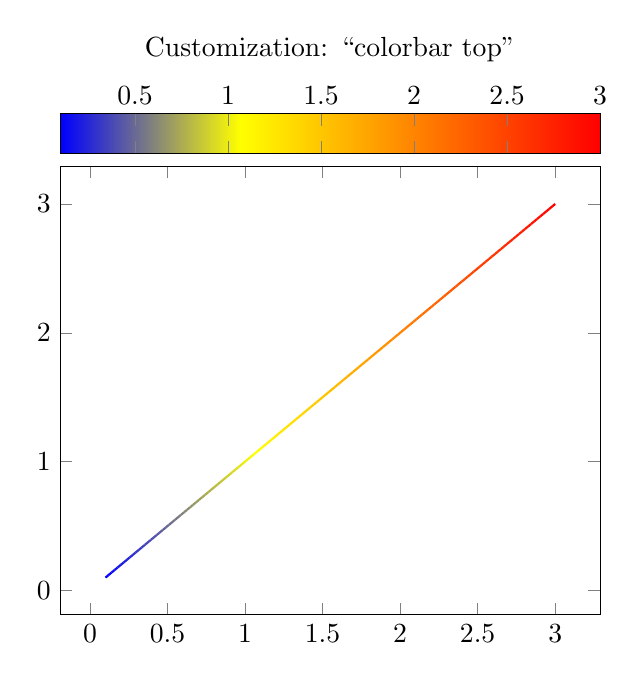
\begin{tikzpicture}
		\begin{axis}[
		colorbar
		horizontal,
		colorbar
		style={
		at={(0.5,1.03)},anchor=south,
		xticklabel
		pos=upper
		},
		title
		style={yshift=1cm},
		title=Customization:
		``colorbar
		top'']
		\addplot[mesh,thick,samples=150,domain=0.1:3]
		{x};
		\end{axis}
		\end{tikzpicture}
		\end{codeexample}
		\begin{codeexample}[]
		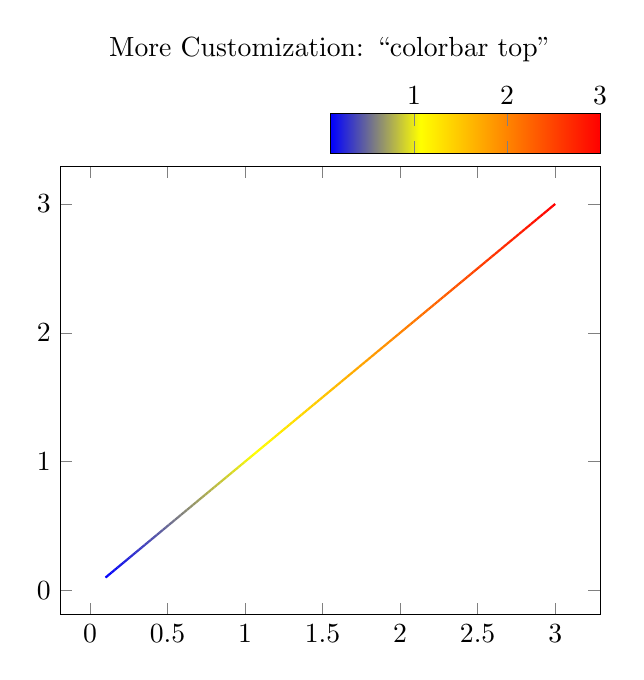
\begin{tikzpicture}
		\begin{axis}[
		colorbar
		horizontal,
		colorbar
		style={
		at={(1,1.03)},anchor=south
		east,
		width=0.5*
		\pgfkeysvalueof{/pgfplots/parent
		axis
		width},
		xticklabel
		pos=upper,
		},
		title
		style={yshift=1cm},
		title=More
		Customization:
		``colorbar
		top'']
		\addplot[mesh,thick,samples=150,domain=0.1:3]
		{x};
		\end{axis}
		\end{tikzpicture}
		\end{codeexample}
		Please
		take
		a
		look
		at
		the
		predefined
		styles
		|colorbar
		right|,
		|colorbar
		left|
		and
		|colorbar
		horizontal|
		for
		more
		details
		about
		configuration
		possibilities
		for
		|every
		colorbar|.
		\paragraph{Remark:}
		A
		color
		bar
		is
		just
		a
		normal
		axis.
		That
		means
		|every
		colorbar|
		can
		contain
		specifications
		where
		to
		place
		tick
		labels,
		extra
		ticks,
		scalings
		and
		most
		other
		features
		of
		a
		normal
		axis
		as
		well
		(except
		nested
		color
		bars).
	}\loadedtable

	\ttfamily
	\pgfplotstablesort[sort cmp={string <}]\loadedtable\loadedtable
	
	%\tracingmacros=2 \tracingcommands=2

	\onecolumn

	\testsubsection{A sorted crap table}

	\pgfplotstabletypeset[column type=l,begin table=\begin{longtable},end table=\end{longtable},verb string type]\loadedtable

	\twocolumn
}
